\documentclass[11pt]{article}
\usepackage{geometry}                
\geometry{letterpaper}                   

\usepackage[utf8]{inputenc}
\usepackage{graphicx}
\usepackage{amssymb}
\usepackage{epstopdf}
\usepackage{natbib}
\usepackage{amssymb, amsmath}
\DeclareGraphicsRule{.tif}{png}{.png}{`convert #1 `dirname #1`/`basename #1 .tif`.png}

%\title{How do participants act during an apéro at ETH}
%\author{Emek Barış Küçüktabak, Francesca Sabena, Emile Courthoud, Hangxi Li}
%\date{date} 

\begin{document}


\input{cover}
\newpage

%%%%%%%%%%%%%%%%%%%%%%%%%%%%%%%%%%%%%%%%%%%%%%%%%

\newpage
\section*{Agreement for free-download}
\bigskip


\bigskip


\large We hereby agree to make our source code for this project freely available for download from the web pages of the SOMS chair. Furthermore, we assure that all source code is written by ourselves and is not violating any copyright restrictions.

\begin{center}

\bigskip


\bigskip


\begin{tabular}{@{}p{1cm}@{}p{8cm}@{}@{}p{8cm}@{}}
\begin{minipage}{1cm}

\end{minipage}
&
\begin{minipage}{6cm}
\vspace{2mm} \large Emek Barış Küçüktabak, Francesca Sabena

 \vspace{\baselineskip}

\end{minipage}
&
\begin{minipage}{4cm}

\large Emile Courthoud, Hangxi Li

\end{minipage}
\end{tabular}


\end{center}
\newpage

%%%%%%%%%%%%%%%%%%%%%%%%%%%%%%%%%%%%%%%



% IMPORTANT
% you MUST include the ETH declaration of originality here; it is available for download on the course website or at http://www.ethz.ch/faculty/exams/plagiarism/index_EN; it can be printed as pdf and should be filled out in handwriting


%%%%%%%%%% Table of content %%%%%%%%%%%%%%%%%

\tableofcontents

\newpage

%%%%%%%%%%%%%%%%%%%%%%%%%%%%%%%%%%%%%%%



\section{Abstract}

\section{Individual contributions}

The project is completed by the cooperation of the whole team: Francesca Sabena, Emek Barış Küçüktabak, Emile Courthoud and Hangxi Li. The research problem and the approach method were decided by a group discussion. Emile contributed to the overall program structure, static wall field, and objective direction; Emek contributed to the arrangement of the table, the person-person force, and table designation; Francesca contributed to the cost function and Hangxi contributed to the food and table forces and position-velocity change. The final report and analysis is written by the whole team. Each team member has contributed in equal amount to the project.

\section{Introduction and Motivations}
The interaction among a group of people has always been a stimulating research topic. The social force model, which was proposed by Helbing\cite{Socialforce,ModificationSocialforce} in order to analyze the pedestrian behaviour, has been proved to be a successful theory to describe the reaction of individuals under the influence of surrounding environment and other people. Recent researches have used the social force model to analyze the behaviour of a pedestrian crowd\cite{crowd1,crowd2,crowd3,traffic3crowd4}, traffic\cite{traffic1,traffic2,traffic3crowd4}, and fish movement\cite{fish}. In this report, we will apply the social force model to simulate the behaviour of the people during the apero. 

An apero is a event for people to gather, chat and eat together. In ETHz, there are many conferences, seminars and talks. After these meetings, an apero usually takes place. People that participate to the apero would at first try to get some food from the buffet table and then gather around the pre-set tables to have a conversation. A real apero in the ETH main building is shown in figure.\ref{fig:apero}.

\begin{figure}[h!]
\centering
\includegraphics[scale=0.3]{apero.jpg}
\caption{Apéro in the ETH}
\label{fig:apero}
\end{figure}

People always tend to follow the shortest path in order to reach their destinations. However, if the environment includes several people, the mutual interaction among them and with the other obstacles will change their desired path; in some peculiar cases, it will even block people's movements for some time. We therefore want to answer the following question: in which situation, given a set of pre-determined parameters, people can get their food and reach tables quickly and successfully during an apero? 
In the report we use the social force model to simulate people's behaviours, assuming that people have their desired movement direction right towards their destinations, but at the same time, their actual movements are affected by the environment and the other people, which are described by different social forces.
\section{Description of the Model}
To simulate the behaviours of the people during an apero, the social force model that has been suggested by Helbing \cite{Socialforce}, is used with some modifications. This model explains the motion of people due to force fields occurring from their destination, obstacles and other people. During an apero, all the people have destinations, which can consist in either the food table or an empty table, and their motion is limited by the walls, tables and the interaction with other people. Thus, this model is suitable for this simulation.
\subsection{Force due to destination}
In real life, people go towards their destination by facing to that point, and trying to move around a constant velocity. This force model acts like a simple proportional controller, where the inputs to this controller are the actual velocity vector and the desired velocity vector.

Desired velocity direction, $\vec{e}_\alpha$ can be defined as in Eq. \ref{develodir}, where as $\vec{r}_\alpha$ denotes the actual position,  $\vec{d}_\alpha$ indicates the position of the destination of the pedestrian $\alpha$,
\begin{equation}
    \vec{e}_\alpha(t):=\frac{\vec{d}_\alpha-\vec{r}_\alpha(t)}{\| \vec{d}_\alpha-\vec{r}_\alpha(t) \|}
\label{develodir}
\end{equation}
So the force on a pedestrian can be written as the multiplication of a constant with the difference of desired velocity vector and the actual velocity vector, as in Eq.\ref{forcedevevec}, where $\vec{v}_\alpha^0$ is the desired speed and $\vec{v}_\alpha$ is the actual speed of the pedestrian $\alpha$,
\begin{equation}
    F_\alpha^0(\vec{v}_\alpha,v_\alpha^0\vec{e}_\alpha) := \frac{1}{\tau}(v_\alpha^0\vec{e}_\alpha-\vec{v}_\alpha)
\label{forcedevevec}
\end{equation}

\subsection{Force due to other pedestrians}
Another important factor that affects the motion of a pedestrian is the behaviour of the other pedestrians. People get uncomfortable due to other people mainly in two cases. First, if somebody is too close to them; second, if somebody is moving towards them.
By using these two facts, the force exerted by a person on other people is defined to be a monotonic decreasing force field with elliptical shape, where the major axis of the ellipse coincides with the velocity vector of the person who exerts the force. The monotonic decreasing part makes the force weaker when the distance between two people increases. The elliptical shape makes the force stronger on the points which are closer to the direction of the person's velocity. This effect can be shown as in Eq.\ref{personforcefield},
\begin{equation}
    \vec{f}_{\alpha\beta}:=-\nabla_{\vec{r}_{\alpha\beta}}V_{\alpha\beta}[b(\vec{r}_{\alpha\beta})]
\label{personforcefield}
\end{equation}
$\vec{f}_{\alpha\beta}$ is the force exerted from pedestrian $\beta$ to pedestrian $\alpha$, $V_{\alpha\beta}$ is any monotonically decreasing function, $\vec{r}_{\alpha\beta}$ is the position of $\beta$ with respect to $\alpha$ and $b$ is the length of the semi minor axis of the described ellipse which is defined in equation Eq.\ref{2b},
\begin{equation}
    2b:=\sqrt{(\|\vec{r}_{\alpha\beta}\|+\|\vec{r}_{\alpha\beta}-v_\beta\Delta t\vec{e}_{\beta}\|)^2-(v_\beta\Delta t)^2}
    \label{2b}
\end{equation}

If the force is defined like this, a person would be effected in the same way both if the other people are behind him/her, both if the people are in front of him/her. To avoid this, the calculated force is multiplied by a coefficient $w$, which is defined as : 
\begin{equation}
    w(\vec{e},\vec{f})=\begin{cases}
    1, & \text{if $\vec{e}\cdot\vec{f}\geq\|\vec{f}\|\cos{\phi}$}.\\
    0, & \text{otherwise}.
  \end{cases}
\end{equation}
where $c$ is taken a value between 0 and 1.

\subsection{Force due to obstacles and walls}
People feel uncomfortable as they get closer to the walls and obstacles. This effect can be visualized as a force coming from the obstacles whose magnitude increases monotonically as the distance between people and obstacles decreases. Thus, similar to the force between people, force due to walls can be described as follows:
\begin{equation}
    \vec{F}_{\alpha B}:=-\nabla_{\vec{r}_{\alpha B}}U_{\alpha B}[b(\|\vec{r}_{\alpha B}\|)]
\end{equation}
where $ \vec{F}_{\alpha B}$ is the force between pedestrian $\alpha$ and obstacle $B$. And $U_{\alpha B}$ is any monotonically decreasing function with respect to distance between pedestrian and obstacle. Details of that function is explained under the implementation section.

\subsection{Total Force}
The resultant force at a time instant on a pedestrian is simply the sum of the force due to objective, the forces exerted by all of the obstacles/walls and the forces from every person in the room. This is shown in Eq[x+6],
\begin{equation}
    \vec{F}_\alpha(t):=\vec{F}_\alpha^0(\vec{v}_\alpha,v_\alpha^0\vec{e}_\alpha)+\sum_\beta\vec{F}_{\alpha\beta}(\vec{e}_\alpha,\vec{r}_\alpha-\vec{r}_\alpha)+\sum_B\vec{F}_{\alpha B}(\vec{e}_\alpha,\vec{r}_\alpha-\vec{r}_\alpha^B)
\end{equation}

\section{Implementation}
\subsection{Social Force Model Algorithm}
Under the description of the model section, it is explained that, it is a good idea to obtain the force from a monotonically decreasing potential field. Due to the fact that as the distance between people increases their interaction effects decrease faster than the distance, an exponentially decreasing potential is used as in Eq.\ref{personpersonpoten}.
\begin{equation}
    V_{\alpha\beta}(b)=V^0_{\alpha\beta}e^{b/\sigma}
    \label{personpersonpoten}
\end{equation}
where, $V^0_{\alpha\beta}$ is taken $2m^2s^{-2}$ and $\sigma=0.2m$. Moreover, the force between two agents is post multiplied by a constant depending on their heading direction and the angle between them. If the angle between the heading direction of a pedestrian $\alpha$ and the position vector of a pedestrian $\beta$ is more than $60^\circ$, the calculated force exerted from $\beta$ to $\alpha$ is multiplied by 0.3 to decrease the effect. One may expect to think that the force exerted from $\alpha$ to $\beta$ to be equal to the force exerted from $\beta$ to $\alpha$. However, this is sometimes not the case. For example, there are 2 people going to a same destination, one in front of the other. While there is a great force exerted from the person in front to the one behind, the force exerted from the person behind to the front one is much less.

\subsection{Wall - person repulsion}
A pedestrian wants to keep a certain distance from the borders of the obstacles in the room, like the walls, doors and pillars.

According to the description provided in the Social Force Model, the influence of the obstacles is modelled by a monotonically decreasing potential field. Focusing on our model, we described the wall-person interaction with a force inversely proportional to the distance between the them.

It must be remarked that the wall is not a point source. To describe the effect of every obstacle in space, we discretized them into several point sources at constant distance. The total repulsion force consists in the superposition of the point source contributions.

\begin{equation}
    F_{\text{wall-person}}=\sum_{i=1}^N\frac{k}{D^2_{p-w,i}}
\end{equation}
where, $D_{p-w,i}$ denotes the distance between a person and the wall point source. According to the simulation outcomes, the value of the proportionality person-wall constant $k$ is set to 0.0003.

The calculation of the point source contributions is numerically expensive. We exploited the fact that the wall effect is constant in time and we saved the wall impact into a file. In order to be able to save it, we discretized the Apero room into a rectangular mesh of points, at which corners the wall repulsion is calculated. The maps containing the force direction, magnitude and orientation is saved into a file, which is opened only once every simulation. 

Finally, the force impact on a person is calculated as the weighted average of the forces applied to the nearest points to a person. The average is weighted on the distance of these points and the person.

We were aware that the discretization procedure introduces a physical inaccuracy. Nevertheless, the error related to the discretization of the walls and of the room becomes negligible when the distance composing the mesh is particularly accurate.

\subsection{Table - person repulsion}
The participants to the Apero usually want to take some food before moving to a table where they can eat and chat. While they move towards the food, the tables become obstacles. Their influence on pedestrian's movement is modelled in the same way of the wall repulsive force, except that the tables are considered point sources.

As we did for the wall repulsion force, we established a table-person constant. We tested several values for this constant and eventually we set $C_t = 0.05$.

\subsection{Path towards the objective}
We assumed that the main objective of every person consists in taking the food as fast as possible and then move to the nearest table. In order to reach these two destinations, the pedestrians try to follow the shortest path.

We modelled the pedestrian's attraction to the objective with a constant pulling force pointing towards the pedestrian's goal. If there are static obstacles like walls between a person and the objective, the pedestrian follows the shortest polygonal route.

\subsection{Destination change}
When people first reach to the Apéro hall, their first destination is the big table with the food on it. After they take their food, they usually want to carry their food to one of the small distributed tables on the hall. They tend to choose the table which is closer, not full and the one with, not more other people, than the capacity of the table goes to the table. In other words, if the maximum number of people that the table can afford is 5, and 7 people already on their way to that table, that person would not try to reach that table, because s/she knows s/he cannot make it. In our algorithm, people choose which table to go with the same logic. Pseudo code of this behavior given in Fig.\ref{fig:sudocode}:

\begin{figure}[ht!]
\centering
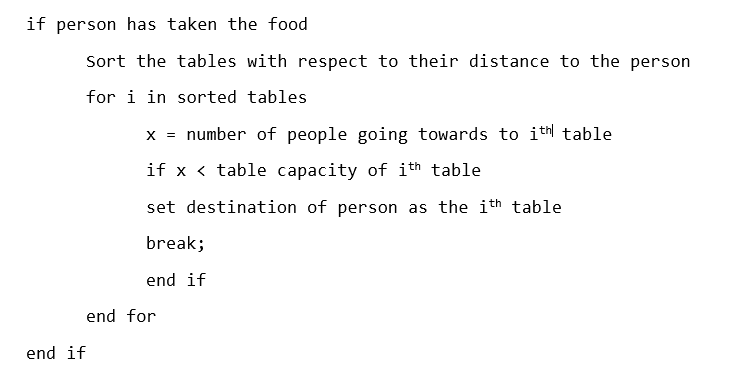
\includegraphics[scale=0.7]{sudocode.png}
\caption{The pseudo code of destination change}
\label{fig:sudocode}
\end{figure}

\section{Simulation Results and Discussion}
In order to simulate and to obtain some results to compare from our model, we implemented 3 functions that return the specific cost of every different simulation.

The 3 parameters that taken into account are:
\begin{itemize}
    \item The time of each participant to reach the final table
    \item The average velocity of each participant
    \item The average total force applied to each participant
\end{itemize}
\hfill\break
\underline{Time cost function}

The time cost function takes into account the time required from each participant to reach the final table. It is the summation of the time to reach the food table (t1) and the time to reach the final table once the food has been taken (t2). The cost related to each person is equal to the total time required to reach the final table, and the cost of the simulation is the mean of the cost of each participant.\\
\underline{Velocity cost function}

The velocity cost function takes into account the average velocity of each participant, in order to penalize the simulations where the participants are stuck and their velocity is equal or close to zero. Since the cost should rise when the velocity is lower, in this function the cost of each participant is equal to $\frac{1}{v}$, where v is the mean velocity of each person. The total cost of the simulation is taken as the mean of the cost of each participant.\\
\underline{Force cost function}

The force cost function takes into account the average force applied to each participant during the entire simulation. The cost of each participant is equal to the total force applied despite the objective force and the total cost is taken as the mean of the cost of each participant.\\

The simulation has been conducted by averaging the simulations with different parameters over 20 attempts each.

The parameters that changed were:
\begin{itemize}
    \item Number of participants
    \item Number of tables
    \item Disposition of tables (Circle or Rectangular)
    \item Distance between the food positions on the buffet table
\end{itemize}

\subsection{Changing the food positions}

The following figures, fig.\ref{fig:foodcostt}, fig.\ref{fig:foodcostv}, fig.\ref{fig:foodcostf} shown are the cost of time, velocity and force if the table's disposition is rectangular or circle. The distance between the food positions varies from 0 to 2.7. In order to simulate the crowding situation, we initialized 72 people starting from both upper corners of the hall (each corner has 36 people), and there are 8 tables with the capacity of 9, so that each person will have his/her seat at the end of the simulation.
\begin{figure}[ht!]
\centering
\includegraphics[scale=0.15]{foodchangecosttime.png}
\caption{The cost of time as varying the food separation}
\label{fig:foodcostt}
\end{figure}

\begin{figure}[ht!]
\centering
\includegraphics[scale=0.15]{foodchangecostv.png}
\caption{The cost of velocity as varying the food separation}
\label{fig:foodcostv}
\end{figure}

\begin{figure}[ht!]
\centering
\includegraphics[scale=0.15]{foodchangecostf.png}
\caption{The cost of force as varying the food separation}
\label{fig:foodcostf}
\end{figure}
The figure.\ref{fig:foodcostt} shows that, under the circle arrangement of table, the cost of time decrease monotonously as the two food positions separate themselves, while in the rectangular table arrangement, the cost of time fluctuates fiercely. The overall pattern of the cost of time indicates that under our social force model, the average time for each person to get their food and reach the tables has no significant correlation with the distance of two food positions.

An interesting phenomenon occurs considering the cost of velocity in figure.\ref{fig:foodcostv}. The cost of velocity still decreases monotonously if table's deposition is circle, but the cost of velocity under rectangular arrangement experiences an down-"U" shape as the distance between two food positions changes. A possible explanation is that when food's separation is around 2, the food points are just below the tables, thus people that have fetched the food will be more likely blocked by the tables, especially when these tables are full.

With circular deposition, the cost of force decreases along with the increase of the food separation. For the rectangular arrangement, the cost of force reaches its minimum when the distance of food locations is 1.

From these three cost functions, we can conclude that for circular table deposition, the foods separate wider, people will be quicker, use less time and experience fewer forces, while if table's arrangement is rectangular, the best food separation distance is around 0.5 to 1, making both food points to be inside of the table lines, but separate a bit.

\section{Summary and Outlook}






\bibliographystyle{unsrt}
\bibliography{references}
\end{document}  
